\documentclass[aspectratio=169,10pt]{beamer}
\usetheme{default}
\usefonttheme{professionalfonts}
\usepackage{booktabs}
\usepackage{graphicx}
\usepackage{tikz}
\usetikzlibrary{arrows.meta,positioning}
\definecolor{ink}{RGB}{24,32,43}
\definecolor{paper}{RGB}{248,246,240}
\definecolor{moss}{RGB}{23,104,89}
\definecolor{sun}{RGB}{210,126,29}
\definecolor{muted}{RGB}{87,98,112}
\setbeamercolor{normal text}{fg=ink,bg=paper}
\setbeamercolor{frametitle}{fg=ink,bg=paper}
\setbeamercolor{structure}{fg=moss}
\setbeamertemplate{navigation symbols}{}
\setbeamertemplate{footline}{\hfill\insertshorttitle\quad\insertframenumber/\inserttotalframenumber\hspace{1.2em}\vspace{.7em}}
\setbeamertemplate{frametitle}{\vspace{.45em}\insertframetitle\par\vspace{.25em}\color{moss}\rule{\textwidth}{.5pt}}
\setbeamerfont{frametitle}{series=\bfseries,size=\Large}
\setbeamerfont{title}{series=\bfseries,size=\LARGE}
\setlength{\leftmargini}{1.1em}
% Right-side exclusion rail keeps the presenter camera off content
\setbeamersize{text margin left=1.0cm,text margin right=4.2cm}
\newcommand{\claim}[1]{\begin{beamercolorbox}[rounded=true,sep=.65em,wd=\linewidth]{block body}\centering\bfseries\color{moss}#1\end{beamercolorbox}}
\newcommand{\smallsource}[1]{\vfill\hfill{\scriptsize\color{muted}#1}}
\title[OpenMP simulation engine]{One loop, one measured limit}
\subtitle{Checksum-verified OpenMP scaling of an independent M2 simulation engine}
\author{COSC3500 --- Milestone 2}
\date{September 2026}

\begin{document}

\begin{frame}
  \titlepage
  \vspace{-1em}
  \claim{Question: how far does one OpenMP optimisation scale before serial CSR rebuilding dominates?}
\end{frame}

\begin{frame}{See the workload first}
\begin{center}
  
\includegraphics[width=.92\linewidth,height=.60\textheight,keepaspectratio]{demo-poster.png}
\end{center}
\vspace{-.4em}
\claim{Blue prey flee red hunters. The clip shows 256 agents; the benchmark uses 100,000.}
\smallsource{\texttt{docs/presentation/demo.mp4}: illustrative engine capture, not benchmark evidence}
\end{frame}

\begin{frame}{The claim is deliberately narrow}
\begin{columns}[T,onlytextwidth]
\column{.49\textwidth}
\textbf{Engine boundary}
\begin{itemize}\itemsep.45em
  \item Deterministic fixed-step state engine
  \item 2D simulation; renderer supplies 2.5D presentation
  \item Scenario selects a kernel and rules
  \item Renderer is outside the timed loop
\end{itemize}
\column{.49\textwidth}
\textbf{Measured M2 workload}
\begin{itemize}\itemsep.45em
  \item Continuous predator--prey kernel
  \item 100,000 agents, 10 fixed steps, radius 80
  \item Seeds 31, 32 and 33
  \item One allocated Rangpur virtual CPU node
\end{itemize}
\end{columns}
\vspace{.65em}
\claim{I am not claiming every scene or kernel has the same speed-up.}
\end{frame}

\begin{frame}{One step, then repeat}
\centering
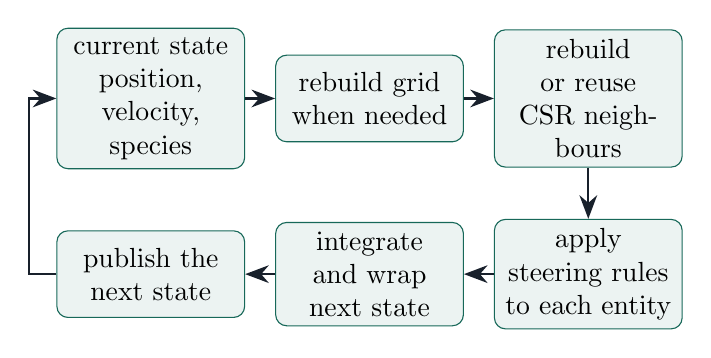
\begin{tikzpicture}[node distance=.65cm and .38cm,box/.style={draw=moss,rounded corners=4pt,fill=moss!8,minimum height=1.1cm,text width=2.15cm,align=center},arrow/.style={-{Stealth[length=3mm]},thick,draw=ink}]
\node[box] (state) {current state\\position, velocity, species};
\node[box,right=of state] (grid) {rebuild grid\\when needed};
\node[box,right=of grid] (csr) {rebuild or reuse\\CSR neighbours};
\node[box,below=of csr] (rule) {apply steering rules\\to each entity};
\node[box,left=of rule] (next) {integrate and wrap\\next state};
\node[box,left=of next] (commit) {publish the\\next state};
\draw[arrow] (state)--(grid); \draw[arrow] (grid)--(csr); \draw[arrow] (csr)--(rule); \draw[arrow] (rule)--(next); \draw[arrow] (next)--(commit);
\draw[arrow] (commit.west) -- ++(-.35,0) |- (state.west);
\end{tikzpicture}
\vspace{.3em}
\begin{columns}[T,onlytextwidth]
\column{.49\textwidth}\textbf{Naive discovery}: $\Theta(n^2)$ candidate tests
\column{.49\textwidth}\textbf{Grid + CSR}: $\Theta(n+m)$, where $m$ is local candidate work
\end{columns}
\vspace{.25em}
\claim{After the final step, hash the state; rendering stays outside the timed loop.}
\end{frame}

\begin{frame}{The optimisation: parallelise only safe per-entity reuse}
\centering
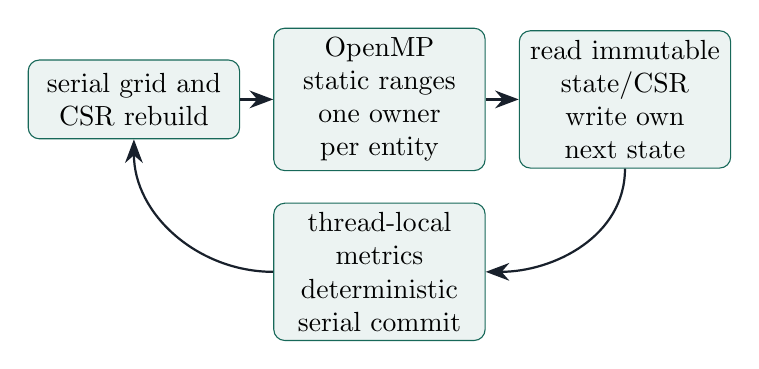
\begin{tikzpicture}[node distance=.40cm and .42cm,box/.style={draw=moss,rounded corners=4pt,fill=moss!8,minimum height=1.0cm,text width=2.45cm,align=center},arrow/.style={-{Stealth[length=3mm]},thick,draw=ink}]
\node[box] (build) {serial grid and\\CSR rebuild};
\node[box,right=of build] (omp) {OpenMP static ranges\\one owner per entity};
\node[box,right=of omp] (write) {read immutable state/CSR\\write own next state};
\node[box,below=of omp] (commit) {thread-local metrics\\deterministic serial commit};
\draw[arrow] (build)--(omp); \draw[arrow] (omp)--(write); \draw[arrow] (write.south) to[out=-90,in=0] (commit.east); \draw[arrow] (commit.west) to[out=180,in=-90] (build.south);
\end{tikzpicture}
\vspace{0em}
\begin{columns}[T,onlytextwidth]
\column{.49\textwidth}\textbf{Invariant}\begin{itemize}\itemsep0em
\item Disjoint entity ownership
\item Immutable current state and CSR
\item Same seed, rule order and checksum oracle
\end{itemize}
\column{.49\textwidth}\textbf{What changes}\begin{itemize}\itemsep0em
\item L7 reuse loop becomes OpenMP work-sharing
\item Grid/CSR rebuild remains serial
\end{itemize}
\end{columns}
\end{frame}

\begin{frame}{How we measured}
\centering
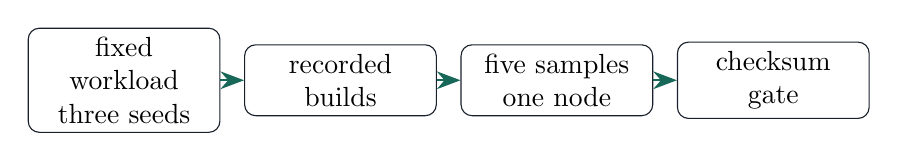
\begin{tikzpicture}[node distance=.25cm and .30cm,box/.style={draw=ink,rounded corners=4pt,fill=white,minimum height=.90cm,text width=2.2cm,align=center},arrow/.style={-{Stealth[length=3mm]},thick,draw=moss}]
\node[box] (a) {fixed workload\\three seeds};
\node[box,right=of a] (b) {recorded builds};
\node[box,right=of b] (c) {five samples\\one node};
\node[box,right=of c] (d) {checksum gate};
\draw[arrow] (a)--(b);\draw[arrow] (b)--(c);\draw[arrow] (c)--(d);
\end{tikzpicture}
\vspace{.4em}
{\setlength{\tabcolsep}{3pt}\renewcommand{\arraystretch}{.94}
\begin{tabular}{@{}lp{.72\linewidth}@{}}
\toprule
Control & Value \\
\midrule
Samples & 1 warm-up + 5 timed samples per tuple \\
Inputs & 3 seeds; checksum must match per seed \\
Placement & one \texttt{vcpu-5} node; CPUs 0--7; one NUMA node \\
Build & GCC 13.3.1; recorded optimisation and OpenMP flags \\
Metric & median ns/entity-update; retain per-seed spread \\
\bottomrule
\end{tabular}
}
\vspace{.45em}
\claim{Only checksum-matched runs enter the charts.}
\end{frame}

\begin{frame}{The measured comparison and its missing baseline}
\centering
\begin{tabular}{lrrrr}
\toprule
Variant & Engine & Threads & ns/entity-update & Ratio \\
\midrule
L0 baseline & M1 & 1 & 358.239 & 1.000$\times$ \\
L7 serial & M2 & 1 & 94.945 & 3.773$\times$ \\
L7 OpenMP & M2 & 1 & 95.185 & 3.759$\times$ \\
L7 OpenMP & M2 & 8 & 52.131 & 6.863$\times$ \\
\bottomrule
\end{tabular}
\vspace{.8em}
\claim{6.863$\times$ crosses from M1 to M2; it cannot measure M2 optimisation alone.}
\vspace{.35em}
\small A same-codebase M2 L0 $\rightarrow$ M2 L7 run is prepared. No M2 optimisation ratio is claimed yet. The parallel comparison starts at OpenMP p1.
\smallsource{Median of seed medians; 3 seeds $\times$ 5 timed samples, workload 100K $\times$ 10 steps}
\end{frame}

\begin{frame}{Measured strong scaling: useful gain, early plateau}
\centering
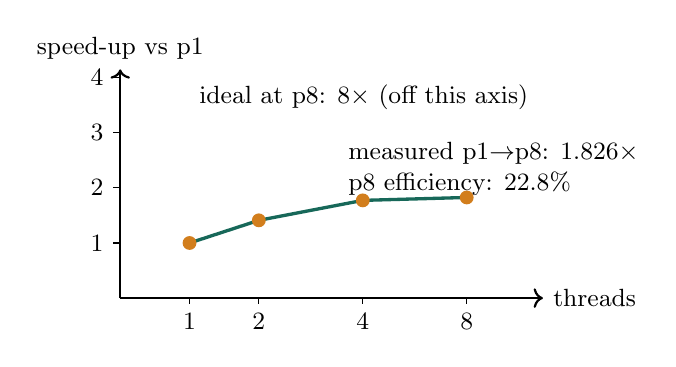
\begin{tikzpicture}[x=.88cm,y=.70cm,font=\small]
  \draw[->,thick] (0,0) -- (6.1,0) node[right]{threads};
  \draw[->,thick] (0,0) -- (0,4.15) node[above]{speed-up vs p1};
  \foreach \x/\l in {1/1,2/2,3.5/4,5/8} \draw (\x,0) -- (\x,-.10) node[below]{\l};
  \foreach \y/\l in {1/1,2/2,3/3,4/4} \draw (0,\y) -- (-.10,\y) node[left]{\l};
  \draw[very thick,moss] plot coordinates {(1,1) (2,1.411) (3.5,1.773) (5,1.826)};
  \foreach \x/\y in {1/1,2/1.411,3.5/1.773,5/1.826} \fill[sun] (\x,\y) circle (2.5pt);
  \node[align=left,anchor=west] at (1.0,3.65) {ideal at p8: $8\times$ (off this axis)};
  \node[align=left,anchor=west] at (3.15,2.35) {measured p1$\rightarrow$p8: $1.826\times$\\p8 efficiency: 22.8\%};
\end{tikzpicture}
\vspace{.05em}
\begin{tabular}{rrrrr}
\toprule
Threads & 1 & 2 & 4 & 8 \\
\midrule
Median ns/entity-update & 95.185 & 67.600 & 53.846 & 52.131 \\
Speed-up vs p1 & 1.000 & 1.410 & 1.773 & 1.826 \\
Efficiency & 100.0\% & 70.5\% & 44.3\% & 22.8\% \\
\bottomrule
\end{tabular}
\smallsource{Ratios are matched per seed then medianed; raw rows retain the seed-level values}
\end{frame}

\begin{frame}{Fixed-density scaling: speed-up holds, per-entity cost rises}
\centering
{\renewcommand{\arraystretch}{.94}
\begin{tabular}{rrrrrr}
\toprule
Agents & p1 ns/unit & p8 ns/unit & $S_8$ & $\eta_8$ & seed range at p8 \\
\midrule
100K & 94.684 & 51.700 & 1.831 & 22.9\% & 51.522--52.261 \\
200K & 101.307 & 53.689 & 1.885 & 23.6\% & 53.006--53.982 \\
400K & 110.450 & 59.458 & 1.855 & 23.2\% & 59.449--59.952 \\
800K & 120.254 & 65.394 & 1.836 & 22.9\% & 65.335--66.287 \\
\bottomrule
\end{tabular}
}
\vspace{.25em}
\begin{columns}[T,onlytextwidth]
\column{.49\textwidth}
\textbf{Fixed density}\par
\small World area grows proportionally with $N$; each run uses 10 fixed steps. $S_8$ stays near 1.8$\times$ across 100K--800K.
\column{.49\textwidth}
\textbf{Weak-scaling check}\par
\small 100K p1 $\rightarrow$ 800K p8: normalized elapsed time is $5.520\times$; weak-scaling efficiency is 18.1\%.
\end{columns}
\vspace{.1em}
\claim{Per-entity time rises with $N$ at both p1 and p8. This is observed behaviour; no hardware cause is asserted because counters were unavailable.}
\smallsource{3 seeds $\times$ 5 timed samples; all serial/OpenMP checksum gates passed}
\end{frame}

\begin{frame}{Why scaling plateaus: instrumented phase evidence}
\begin{columns}[T,onlytextwidth]
\column{.48\textwidth}
\textbf{At p8, median diagnostic time}
\begin{itemize}\itemsep.4em
  \item CSR rebuild: about 33.5 ms (75.8\%)
  \item CSR reuse/publish: about 10.6 ms (24.0\%)
  \item The parallel loop shrinks; rebuild does not
\end{itemize}
\column{.48\textwidth}
\textbf{Inside the serial rebuild}
\begin{itemize}\itemsep.4em
  \item grid/count traversal: about 14.0 ms (42\%)
  \item second fill traversal: about 10.8 ms (32\%)
  \item residual allocation/prefix work: about 8.7 ms (26\%)
\end{itemize}
\end{columns}
\vspace{.7em}
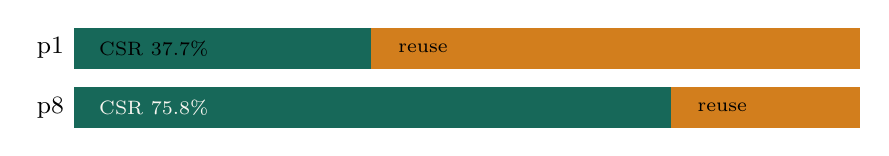
\begin{tikzpicture}[x=.10cm,y=.75cm,font=\small]
\node[anchor=east] at (0,1) {p1}; \node[anchor=east] at (0,0) {p8};
\fill[moss] (0,.65) rectangle (37.7,1.35); \fill[sun] (37.7,.65) rectangle (99.9,1.35);
\fill[moss] (0,-.35) rectangle (75.8,.35); \fill[sun] (75.8,-.35) rectangle (99.8,.35);
\node[anchor=west,font=\scriptsize] at (2,1) {CSR 37.7\%};
\node[anchor=west,font=\scriptsize,text=paper] at (2,0) {CSR 75.8\%};
\node[anchor=west,font=\scriptsize] at (40,1) {reuse};
\node[anchor=west,font=\scriptsize] at (78,0) {reuse};
\end{tikzpicture}
\vspace{.35em}
\claim{This is an instrumented diagnostic build: its milliseconds explain the shape but are not comparable to release timings.}
\end{frame}

\begin{frame}{Decision: optimise the rebuild next, but only after an A/B gate}
\begin{columns}[T,onlytextwidth]
\column{.48\textwidth}
\textbf{Evidence-supported next candidate}
\begin{itemize}\itemsep.25em
  \item Avoid the second CSR fill traversal when a bounded scratch edge list can safely retain accepted pairs
  \item Preserve pair order and checksum
  \item Fall back to the existing traversal when the bounded scratch space is full
\end{itemize}
\column{.48\textwidth}
\textbf{Do not claim it yet}
\begin{itemize}\itemsep.25em
  \item The CSR candidate A/B has no validated result here
  \item Promote only with interleaved, checksum-matched p1/p2/p4/p8 runs
  \item Reject a gain that is not stable across all three seeds
\end{itemize}
\end{columns}
\vspace{.25em}
\claim{CUDA, MPI and hand-written AVX remain unmeasured for this workload.}
\end{frame}

\begin{frame}{Validity, limits and reproducibility}
\begin{columns}[T,onlytextwidth]
\column{.49\textwidth}
\textbf{What this establishes}
\begin{itemize}\itemsep.35em
  \item Independent M2 executable, not M1 reuse
  \item Exact final state per seed across serial and thread counts
  \item Repeated one-node strong-scaling evidence
  \item A measured explanation for the p8 plateau
\end{itemize}
\column{.49\textwidth}
\textbf{What it does not establish}
\begin{itemize}\itemsep.35em
  \item All scenes, densities or initial conditions
  \item Multi-node, GPU or SIMD speed-up
  \item Hardware-counter attribution: \texttt{perf stat} was unavailable on this allocation
  \item A speed-up for the unvalidated CSR candidate
\end{itemize}
\end{columns}
\vspace{.7em}
\smallsource{Raw data: \texttt{results/profile/run-20260924T110021Z-rG8ANs}; phase data: \texttt{results/profile/phase-615532}}
\end{frame}

\begin{frame}{Conclusion}
\begin{enumerate}\itemsep.42em
  \item Static ownership preserved each seed's checksum and gave $1.826\times$ at 8 threads
  \item At p8, serial CSR rebuild occupied 75.8\% of instrumented time; more workers offer little until that changes
  \item Test the bounded scratch candidate against the original binary; reject it if memory or p1 cost outweighs p8 benefit
\end{enumerate}
\vspace{.7em}
\textbf{AI disclosure}\par
\small Generative AI assisted implementation, data checks and slide drafting. I will independently review the final evidence and defend every claim in the interview.
\vspace{.55em}
\claim{Next test: the bounded CSR candidate against the original M2 binary.}
\end{frame}

\end{document}
